\subsection{Выборочные коэффициенты корреляции}
	\begin{table}[H]
		\centering
		\begin{tabular}{| c | c | c | c |}
			
			\hline
			$\rho=0$  & $r$      & $r_S$  & $r_Q$ \\
			\hline
			$E(z)$    & -0.01 & 0.002 & 0.0   \\
			$E(z^2)$  & 0.026 & 0.024 & 0.04  \\
			$D(z)$    & 0.051 & 0.051 & 0.051 \\
			\hline
			$\rho=0.5$ & $r$      & $r_S$  & $r_Q$ \\
			\hline
			$E(z)$    & 0.516 & 0.488 & 0.4   \\
			$E(z^2)$    & 0.267 & 0.239 & 0.16  \\
			$D(z)$      & 0.031 & 0.033 & 0.045 \\
			\hline
			$\rho=0.9$  & $r$      & $r_S$  & $r_Q$ \\
			\hline
			$E(z)$    & 0.903 & 0.88  & 0.8   \\
			$E(z^2)$    & 0.816 & 0.774 & 0.64  \\
			$D(z)$      & 0.003 & 0.005 & 0.028 \\
			\hline
			
		\end{tabular}{}
		\caption{Двумерное нормальное распределение, n = 20}
		\label{tab:n20}
	\end{table}
	
	
	\begin{table}[H]
		\centering
		\begin{tabular}{| c | c | c | c |}
			
			\hline
			$\rho = 0$ & $r$      & $r_S$  & $r_Q$ \\
			\hline
			$E(z)$    & -0.013 & -0.01 & 0.0   \\
			$E(z^2)$  & 0.008  & 0.007 & 0.004 \\
			$D(z)$    & 0.015  & 0.015 & 0.016 \\
			\hline
			$\rho = 0.5$ & $r$      & $r_S$  & $r_Q$ \\
			\hline
			$E(z)$    & 0.497 & 0.47  & 0.333 \\
			$E(z^2)$    & 0.247 & 0.221 & 0.111 \\
			$D(z)$      & 0.009 & 0.011 & 0.014 \\
			\hline
			$\rho = 0.9$ & $r$      & $r_S$  & $r_Q$ \\
			\hline
			$E(z)$    & 0.9   & 0.885 & 0.733 \\
			$E(z^2)$    & 0.81  & 0.784 & 0.538 \\
			$D(z)$      & 0.001 & 0.001 & 0.009 \\
			\hline
			
		\end{tabular}{}
		\caption{Двумерное нормальное распределение, n = 60}
		\label{tab:n60}
	\end{table}
	
	
	
	\begin{table}[H]
		\centering
		\begin{tabular}{| c | c | c | c |}
			
			\hline
			$\rho = 0$ & $r$      & $r_S$  & $r_Q$ \\
			\hline
			$E(z)$    & -0.005 & -0.004 & 0.0   \\
			$E(z^2)$  & 0.005  & 0.005  & 0.006 \\
			$D(z)$    & 0.01   & 0.01   & 0.01  \\
			\hline
			$\rho = 0.5$ & $r$      & $r_S$  & $r_Q$ \\
			\hline
			$E(z)$    & 0.496 & 0.477 & 0.32  \\
			$E(z^2)$    & 0.246 & 0.227 & 0.102 \\
			$D(z)$      & 0.006 & 0.007 & 0.009 \\
			\hline
			$\rho = 0.9$ & $r$      & $r_S$  & $r_Q$ \\
			\hline
			$E(z)$    & 0.9  & 0.887 & 0.72  \\
			$E(z^2)$    & 0.81 & 0.787 & 0.518 \\
			$D(z)$      & 0.0  & 0.001 & 0.005 \\
			\hline
			
		\end{tabular}{}
		\caption{Двумерное нормальное распределение, n = 100}
		\label{tab:n100}
	\end{table}
	
	
	\begin{table}[H]
		\centering
		\begin{tabular}{| c | c | c | c |}
			
			\hline
			$size = 20$ & $r$      & $r_{S}$ & $r_{Q}$ \\
			\hline
			$E(z)$    & 0.796 & 0.767 & 0.6   \\
			$E(z^2)$    & 0.633 & 0.588 & 0.36  \\
			$D(z)$      & 0.038 & 0.013 & 0.009 \\
			\hline
			$size = 60$ & $r$      & $r_{S}$ & $r_{Q}$ \\
			\hline
			$E(z)$    & 0.793 & 0.772 & 0.6   \\
			$E(z^2)$    & 0.629 & 0.596 & 0.36  \\
			$D(z)$      & 0.011 & 0.004 & 0.003 \\
			\hline
			$size = 100$ & $r$      & $r_{S}$ & $r_{Q}$ \\
			\hline
			$E(z)$    & 0.793 & 0.775 & 0.56  \\
			$E(z^2)$     & 0.63  & 0.6   & 0.314 \\
			$D(z)$       & 0.007 & 0.002 & 0.002 \\
			\hline
			
		\end{tabular}{}
		\caption{Смесь нормальных распределений}
		\label{tab:mix_normal}
	\end{table}
	
\subsection{Эллипсы рассеивания}
	
	\begin{figure}[H]
		\centering
		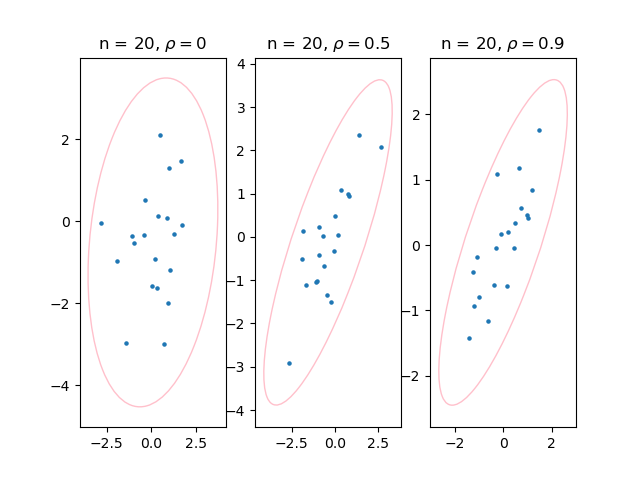
\includegraphics[width = 10cm, height = 8cm]{pics/n20.png}
		\caption{Двумерное нормальное распределение, n = 20}
		\label{fig:n20}
	\end{figure}
	
	\begin{figure}[H]
		\centering
		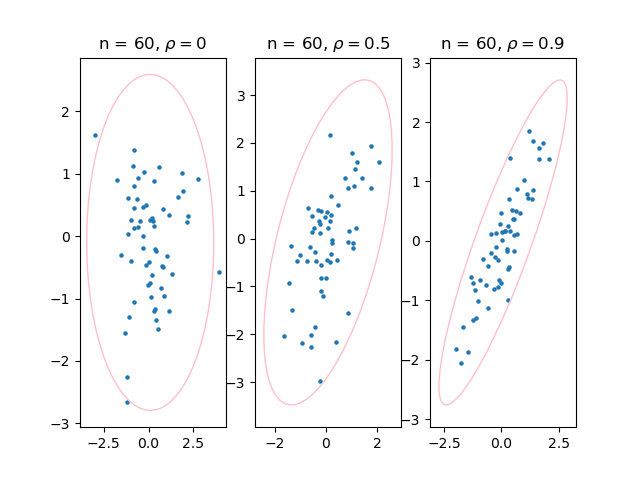
\includegraphics[width = 10cm, height = 8cm]{pics/n60.png}
		\caption{Двумерное нормальное распределение, n = 60}
		\label{fig:n60}
	\end{figure}

	\begin{figure}[H]
		\centering
		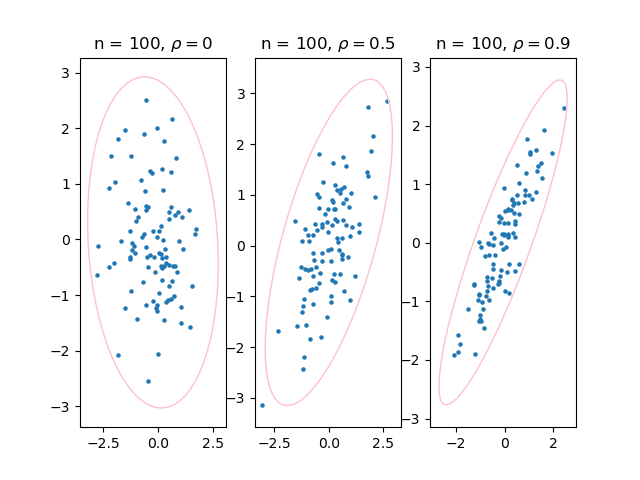
\includegraphics[width = 10cm, height = 8cm]{pics/n100.png}
		\caption{Двумерное нормальное распределение, n = 100}
		\label{fig:n100}
	\end{figure}

	
\subsection{Оценки коэффициентов линейной регрессии}

Метрика удаленности: $distance = \sum_{i=0}^{n}(y_{model}[i]-y_{regr}[i])^2$
\subsubsection{Выборка без возмущений}
\begin{enumerate}
	\item{Критерий наименьших квадратов:}
	$\hat{a}\approx 1.91$, $\hat{b}\approx 1.87$
	\item{Критерий наименьших модулей:}
	$\hat{a}\approx 1.84$, $\hat{b}\approx 1.71$
\end{enumerate}
\begin{figure}[H]
	\centering
	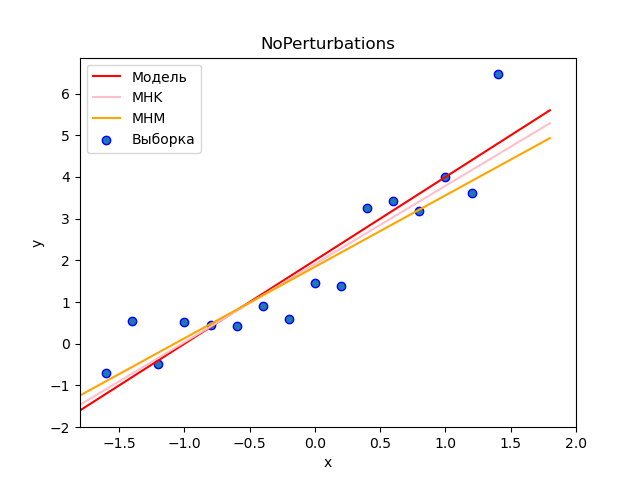
\includegraphics[width = 10cm, height = 8cm]{pics/NoPerturbations.png}
	\caption{Выборка без возмущений}
	\label{w/o_pert}
\end{figure}
МНК distance = 0.49 \\
МНМ distance = 2.31

\subsubsection{Выборка с возмущениями}
\begin{enumerate}
	\item{Критерий наименьших квадратов:}
	$\hat{a}\approx 1.91$, $\hat{b}\approx 0.29$
	\item{Критерий наименьших модулей:}
	$\hat{a}\approx 1.62$, $\hat{b}\approx 1.88$
\end{enumerate}
\begin{figure}[H]
	\centering
	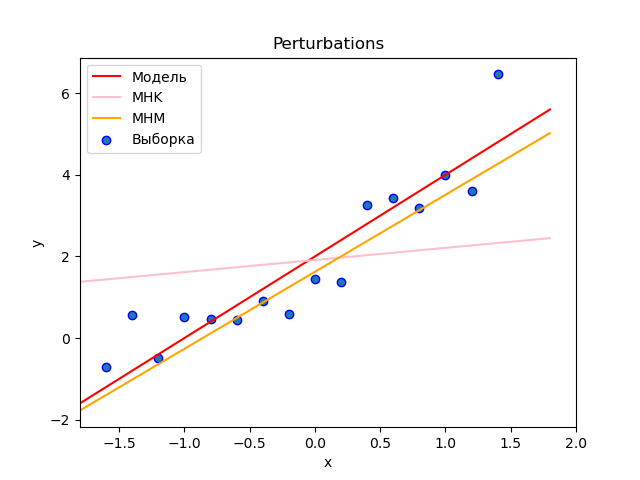
\includegraphics[width = 10cm, height = 8cm]{pics/Perturbations.png}
	\caption{Выборка с возмущениями}
	\label{w_pert}
\end{figure}
МНК distance = 66.24 \\
МНМ distance = 2.97

\subsection{Проверка гипотезы о законе распределения генеральной совокупности. Метод хи-квадрат}
Метод максимального правдоподобия:
\newline
$\hat{\mu} \approx 0.08, \hat{\sigma} \approx 1.02$
\newline
Критерий согласия $\chi^{2}$:
\newline
Количество промежутков k = 6
\newline
Уровень значимости $\alpha$= 0.05
\newline
Тогда квантиль $\chi^{2}_{1-\alpha}(k-1)$ = $\chi^{2}_{0.95}(5)$. Из таблицы [3, с. 358] $\chi^{2}_{0.95}(5) \approx 11.07$. 
\begin{table}[H]
	\centering
	\begin{tabular}{| c | c | c | c | c | c | c |}
		\hline
		$i$ & $limits$         &   $n_i$ &    $p_i$ &   $np_i$ &   $n_i - np_i$ &   $\frac{(n_i-np_i)^2}{np_i}$ \\
		\hline
		1 & [$-\infty$, -1.1] &    13 & 0.1357 &  13.57 &        -0.57 &                        0.02 \\
		2 & [-1.1, -0.55]  &    19 & 0.1555 &  15.55 &         3.45 &                        0.77 \\
		3 & [-0.55, 0.0]   &    14 & 0.2088 &  20.88 &        -6.88 &                        2.27 \\
		4 & [0.0, 0.55]    &    25 & 0.2088 &  20.88 &         4.12 &                        0.81 \\
		5 & [0.55, 1.1]    &    12 & 0.1555 &  15.55 &        -3.55 &                        0.81 \\
		6 & [1.1,  $\infty$]   &    17 & 0.1357 &  13.57 &         3.43 &                        0.87 \\
		$\sum$ & $-$              &   100 & 1      & 100    &        -0    &                        5.55 \\
		\hline
	\end{tabular}
	\caption{ Вычисление $\chi^{2}_{B}$ при проверке гипотезы $H_{0}$ о нормальном законе распределения $N(x,\hat{\mu}, \hat{\sigma})$}
	\label{tab:normal_chi_2}
\end{table} 

Сравнивая $\chi^{2}_{B} = 5.55$ и $\chi^{2}_{0.95}(5) \approx 11.07$, видим, что $\chi^{2}_{B} < \chi^{2}_{0.95}(5)$.

\begin{table}[H]
	\centering
	\begin{tabular}{| c | c | c | c | c | c | c |}
		\hline
		$i$ & $limits$         &   $n_i$ &    $p_i$ &   $np_i$ &   $n_i - np_i$ &   $\frac{(n_i-np_i)^2}{np_i}$ \\
		\hline
		1 & [$-\infty$, -1.1] &     2 & 0.1357 &   2.71 &        -0.71 &                        0.19 \\
		2 & [-1.1, -0.55]  &    	 2 & 0.1555 &   3.11 &        -1.11 &                        0.4  \\
		3 & [-0.55, 0.0]   &     6 & 0.2088 &   4.18 &         1.82 &                        0.8  \\
		4 & [0.0, 0.55]    &    7 & 0.2088 &   4.18 &         2.82 &                        1.91 \\
		5 & [0.55, 1.1]    &     1 & 0.1555 &   3.11 &        -2.11 &                        1.43 \\
		6 & [1.1,  $\infty$]   &    2 & 0.1357 &   2.71 &        -0.71 &                        0.19 \\
		$\sum$ & $-$              &    20 & 1      &  20    &        -0    &                        4.91 \\
		\hline
	\end{tabular}
	\caption{ Вычисление $\chi^{2}_{B}$ при проверке гипотезы $H_{0}$ о законе распределения $L(x,\hat{\mu}, \hat{\sigma})$, $n=20$},
	\label{tab:laplace_chi_2}
\end{table}
Сравнивая $\chi^{2}_{B} = 4.91$ и $\chi^{2}_{0.95}(5) \approx 11.07$, видим, что $\chi^{2}_{B} < \chi^{2}_{0.95}(5)$.

\subsection{Доверительные интервалы для параметров нормального распределения}
\begin{table}[H]
	\centering
	\begin{tabular}{| c | c | c |}
		\hline
		n = 20   &  $m$  & $\sigma$\\ \hline
		&  -0.69 < $m$ < 0.19 & 0.71 < $\sigma$ < 1.37 \\ \hline
		&   &   \\ \hline
		n = 100   &  $m$  & $\sigma$\\ \hline
		& -0.28 < $m$ < 0.12 & 0.88 < $\sigma$ < 1.16 \\
		\hline
	\end{tabular}
	\caption{Доверительные интервалы для параметров нормального распределения}
	\label{tab:interv_simple}
\end{table}

\subsection{Доверительные интервалы для параметров произвольного распределения. Асимптотический подход}
\begin{table}[H]
	\centering
	\begin{tabular}{| c | c | c |}
		\hline
		n = 20   &  $m$  & $\sigma$\\ \hline
		&  -0.65 < $m$ < 0.15 & 0.8 < $\sigma$ < 1.1 \\ \hline
		&   &   \\ \hline
		n = 100   &  $m$  & $\sigma$\\ \hline
		& -0.28 < $m$ < 0.11 & 0.94 < $\sigma$ < 1.07 \\
		\hline
	\end{tabular}
	\caption{Доверительные интервалы для параметров произвольного распределения. Асимптотический подход}
	\label{tab:interv_asimpt}
\end{table}